%++++++++++++++++++++++++++++++++++++++++
% Don't modify this section unless you know what you're doing!
\documentclass[letterpaper,12pt]{article}
\usepackage{tabularx} % extra features for tabular environment
\usepackage{amsmath}  % improve math presentation
\usepackage{graphicx} % takes care of graphic including machinery
\usepackage{float}
\usepackage[margin=1in,letterpaper]{geometry} % decreases margins
\usepackage{cite} % takes care of citations
\usepackage[final]{hyperref} % adds hyper links inside the generated pdf file
\hypersetup{
	colorlinks=true,       % false: boxed links; true: colored links
	linkcolor=blue,        % color of internal links
	citecolor=blue,        % color of links to bibliography
	filecolor=magenta,     % color of file links
	urlcolor=blue         
}
%++++++++++++++++++++++++++++++++++++++++


\begin{document}

\title{555 Timer Mini-Project Lab Report}
\author{Pradyunn Vikram Kale}
\date{\today}
\maketitle

\section{Introduction}

The 555 Timer was originally designed in 1971 by Hans Camenzind, a swiss electronics engineer employed by Signetics in California. 
He spent months getting the 555 Timer to its final design. 
The 555 timer is simple to use, and reliable in a wide array of applications. 
For all of its applications, it is used in one of 3 modes. 
Monostable, astable, and bistable mode. With these modes, we can make circuits like PWM motor controllers, security alarms, audio generators etc. 
The objective of this project is to learn how 555 timers work and to build something cool out of them. I am interested in building a PWM generator using the 555 timers, as this connects to motor control, something I will be using a lot within GNC. 

\section{Theory}

\begin{figure}[H]
	\centering	
	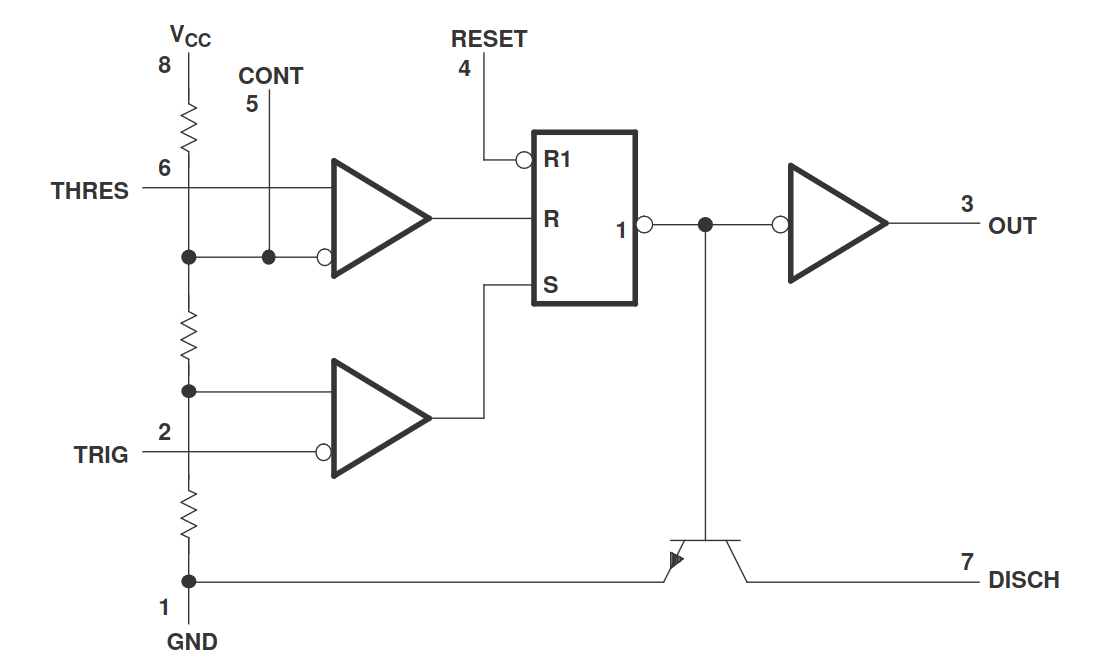
\includegraphics[width=0.8\columnwidth]{555_timer_diagram}
	\caption{
		\label{fig:internaldiagram}
		555 Timer Internal Schematic
	}
\end{figure}

The main components inside the 555 timer are 2 comparators and an SR flip flop in cooperation with a voltage divider. In short, the 555 timer works by using a voltage divider and setting the voltage of specific nodes. 
For example, when looking at the diagram, the node after the first resistor from ground is $\frac{1}{3}V_{cc}$, and then the node after the 2nd resistor from ground is $\frac{2}{3}V_{cc}$. 
The lower comparator uses $\frac{1}{3}V_{cc}$ as a reference, when the trigger voltage falls below $\frac{1}{3}V_{cc}$, the comparator will output HIGH. 
This then asserts SET on the flip flop, which then sets Q to HIGH. 
Since the output is wired to $\overline{Q}$, the output will be LOW. 
The upper comparator uses $\frac{2}{3}V_{cc}$ as a reference. 
If the threshold voltage falls under $\frac{2}{3}V_{cc}$ then RESET will be asserted, setting Q to LOW.
Since the output is connected to $\overline{Q}$, the output will be HIGH.

\begin{figure}[H]
	\centering
	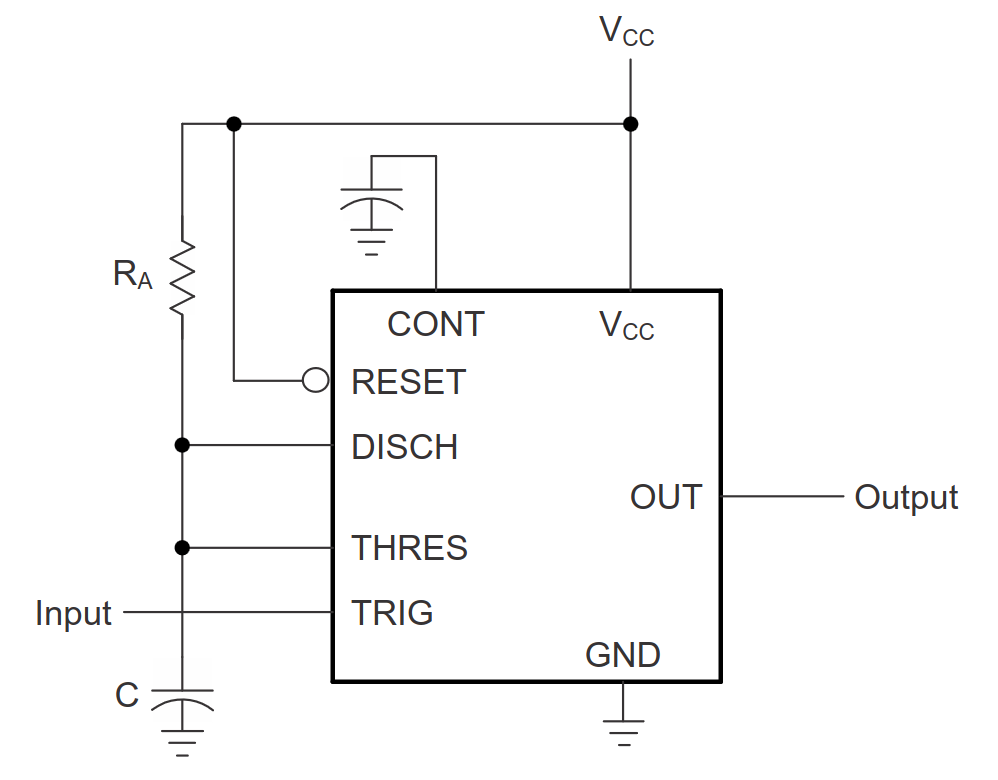
\includegraphics[width=0.8\columnwidth]{555_timer_monostable_diagram.png}
	\caption{
		\label{fig:monostablediagram}
		555 Timer Monostable Mode Schematic
	}
\end{figure}

Monostable Mode of operation is a "one-shot" mode. So on input, monostable mode will make one pulse, and then sleep until another
input is asserted. The equation for the length of the pulse is given below

$$t_w = 1.1 \times R_A C$$

\begin{figure}[H]
	\centering
	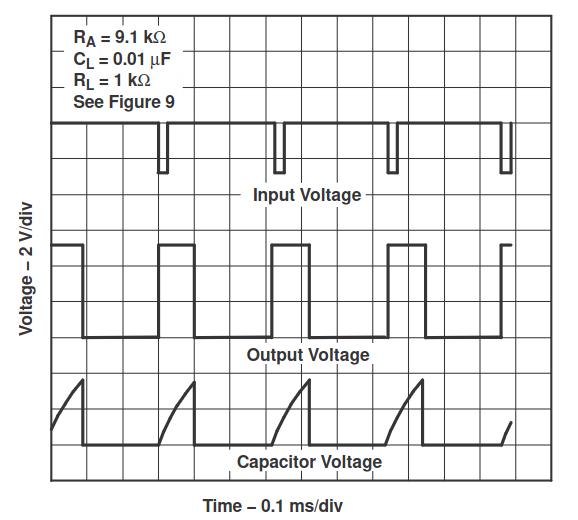
\includegraphics[width=0.8\columnwidth]{555_timer_monostable_signals.png}
	\caption{
		\label{fig:monostablesignals}
		555 Timer Monostable Mode Signals
	}
\end{figure}

We see this equation, especially when looking at the signals for the 555 timer on monostable mode, in \textbf{Figure \ref{fig:monostablesignals}}. 
You can see when the input is asserted when it is pulled low, and based on the equation $t_w = 1.1 \times R_A C$ with $R_A = 9.1$ k$\Omega$ and $C = 0.01$ $\mu$F. 
This gives us $t_w = 1.1 \times (9.1 k\Omega) (0.01 \mu F) = (0.1 \times 10^{-4})$s or 0.1ms, which is seen in the waveforms below. 
You can imagine how the waveforms may differ with different values of $R_a$ and $C$. Another interesting thing is how the capactior voltage drops down when the input is asserted, and then charges back up according to the differential equation governing its behavior.

\begin{figure}[H]
	\centering
	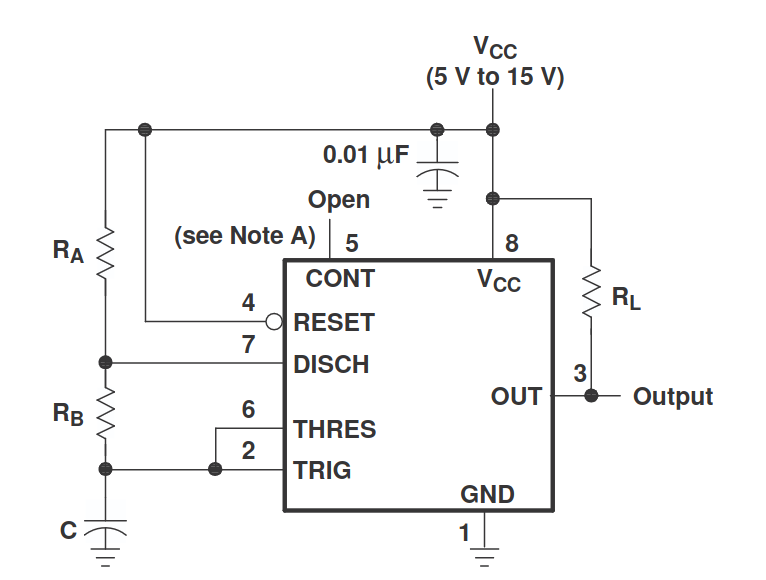
\includegraphics[width=0.8\columnwidth]{555_timer_astable_diagram.png}
	\caption{
		\label{fig:astablediagram}
		555 Timer Astable Mode Schematic 
	}
\end{figure}

Astable Mode is an "oscillation" mode, when the input is asserted, the output will pulse repeatedly with a period of $T = t_H + t_L \cong 0.693 \times (R_A + 2R_B) \times C$, where $t_H \cong 0.693 \times (R_A + R_B) \times C$ and $t_L \cong 0.693 \times R_B \times C$. The placement of the resistors and capacitors are shown in \textbf{Figure \ref{fig:astablediagram}}, which is the schematic for low oscillation mode.
Where $t_H$ and $t_L$ both denote "time HIGH" and "time LOW". The duty cycle of the circuit is defined to be the amount of time the output is HIGH relative to the period of oscillation. The duty cycle equation is simply given by $\frac{t_H}{t_H + t_L} = \frac{R_A + R_B}{R_A + 2R_B}$.

\begin{figure}[H]
	\centering
	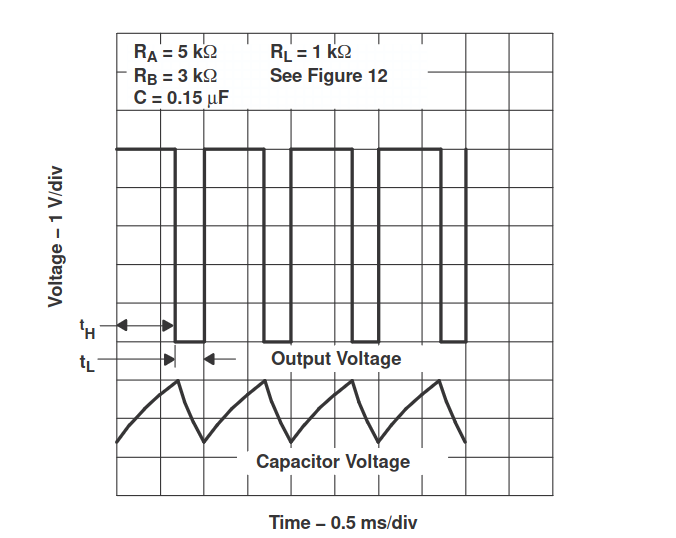
\includegraphics[width=0.8\columnwidth]{555_timer_astable_signals.png}
	\caption{
		\label{fig:astablesignals}
		555 Timer Astable Mode Signals 
	}
\end{figure}

In \textbf{Figure \ref{fig:astablesignals}}. We see how the capacitor voltage and the output signal changes over time. As we can see,
there is a period of oscillation obeying the equations stated above. What is interesting is that as soon as the capacitor charges back up
to $V_{cc}$ it then immediately discharges back to GND. This is because the trigger itself is connected to the capacitor.

\section{Experimental Procedure}

\begin{figure}[H]
	\centering
	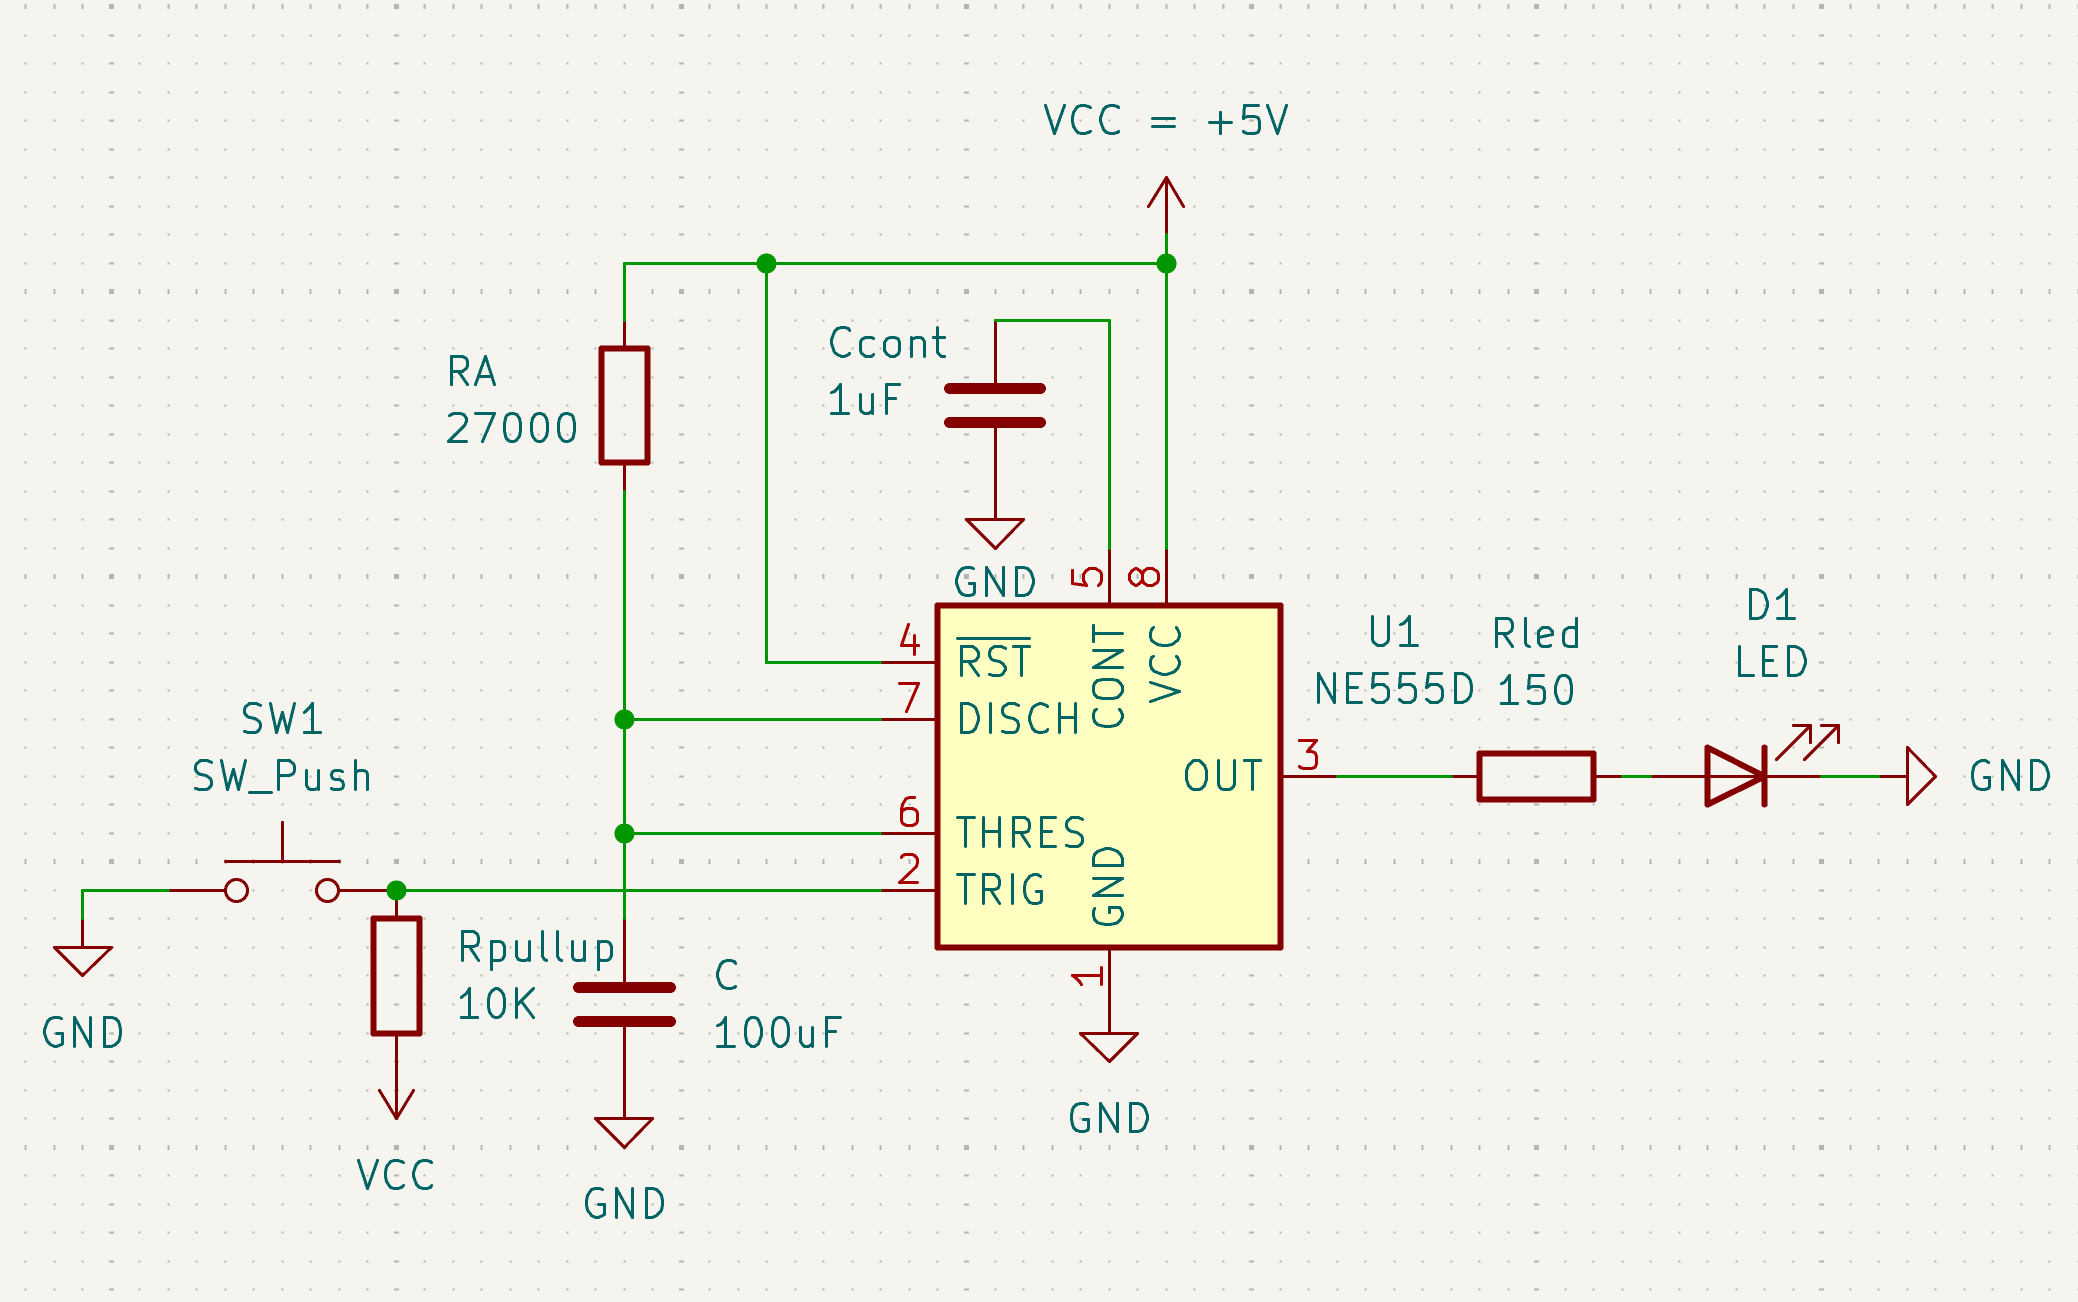
\includegraphics[width=0.8\columnwidth]{experimental_monostable.png}
	\caption{
		\label{fig:experimental_monostable}
		555 Timer Monostable Experiment Schematic
	}
\end{figure}

In order to calculate the amount of time we want the pulse to be on, we need to use the formula $t_w = 1.1 \times R_A C$, since we are targetting a 3 second pulse on, we get the equaton $3 = 1.1 \times R_A C$, simplifying we get that $R_A C = 2.7\overline{27}$, since we are given $100\mu$F capacitors, we can then get that $R_A = \frac{2.7\overline{27}}{100 \times 10^{-6}} \approx 27k\Omega$. 

When building the circuit, I started with setting up the power rails on my breadboard, this allows me to make my circuit very organized on my breadboard. 
Since I connected my power rails, I first connected my power pins ($V_{cc}$ and GND). With those I connected pins that used those signals directly (those being RESET and CONTINUITY).
I connected an LED to the OUTPUT pin so I could see the output. After that I went by the schematic. 
I started with setting up the $R_A$ resistor and the C capacitor as those connections are 
related to 2 of the pins (those being the DISCHARGE and THRESHOLD pins).
I finally connected a push-button to the TRIGGER pin. I made sure to have a pull-up resistor because I do not want my input to be floating
as this can cause erratic behavior in my circuit. The reason I use a pull-up is because the OUTPUT is HIGH when INPUT is LOW. 

\begin{figure}[H]
	\centering
	\includegraphics[width=0.8\columnwidth]{experimental_astable.png}
	\caption{
		\label{fig:experimental_astable}
		555 Timer Astable Experiment Schematic
	}
\end{figure}

In order to get a 60\% duty cycle and a period of 2 seconds. We need to use the equations for $t_H$ and $t_L$. Since we know that
$t_H \cong 0.693 \times (R_A + R_B) \times C = 1.2$ and $t_L \cong 0.693 \times R_B \times C = 0.8$. In both of these equations, we
can divide both sides by $0.693$ to get $1.7316 = (R_A + R_B) \times C$ and $1.1544 = R_B \times C$. I will just use $C = 100\mu F$ because
I have that capacitor available in my kit. This leaves me with $R_B = 11544\Omega$ and $R_A + R_B = 17316\Omega$, using the value we have 
for $R_B$, we get that $R_A = 5772\Omega$. Since we do not have these exact values, for $R_A$ I will be using a $5.6k\Omega$ resistor and 
or $R_B$ I will be using a $12k\Omega$ resistor. This will give us a duty cycle of approximately 60\% over a 2 second period. $f = \frac{1}{T} = 0.5$ Hz where $T = t_H + t_L = 2$.

In order to get a 75\% duty cycle and a period of 1 second. We need to use the equations for $t_H$ and $t_L$. Since we know that $t_H \cong 0.693 \times (R_A + R_B) \times C = 0.75$ and $t_L \cong 0.693 \times R_B \times C = 0.25$. I am going to start with making $C = 100\mu F$
because I have that capacitor available in my kit. This gives the equations $0.75 = (0.693 \times 100 \times 10^{-6}) (R_A + R_B)$ and $0.25 = (0.693 \times 100 \times 10^{-6}) (R_B)$, isolating for $R_B$ in the 2nd equation we get $R_B = 3607\Omega$. Isolating for $R_A$ in the first equation we get $R_A = 7215\Omega$. $f = \frac{1}{T} = 1$ Hz where $T = t_H + t_L = 1$.

Since I already had the 555 Timer monostable cirucit built, I started with whatever I had there. As you can see, since I was given
that circuit to start out with, connecting the rest of the circuit to make it astable circuit. I first took out the input as I no longer needed the input (since the astable circuit will oscillate on its own).


\section{Results and Discussion}

For the monostable mode, the theoretical result is what I have calculated above. However since we are not using a resistor with a 
repeating decimal, I will recalculate the theoretical value of the pulse based on the selection of resistors.
$t_w = 1.1 \times 27000 \times 100\mu F = 2.97s$.



\section{Conclusion and Reference}
Here you briefly summarize your findings.

%++++++++++++++++++++++++++++++++++++++++
% References section will be created automatically 
% with inclusion of "thebibliography" environment
% as it shown below. See text starting with line
% \begin{thebibliography}{99}
% Note: with this approach it is YOUR responsibility to put them in order
% of appearance.

\begin{thebibliography}{99}

\bibitem{melissinos}
A.~C. Melissinos and J. Napolitano, \textit{Experiments in Modern Physics},
(Academic Press, New York, 2003).

\bibitem{Cyr}
N.\ Cyr, M.\ T$\hat{e}$tu, and M.\ Breton,
% "All-optical microwave frequency standard: a proposal,"
IEEE Trans.\ Instrum.\ Meas.\ \textbf{42}, 640 (1993).

\bibitem{Wiki} \emph{Expected value},  available at
\texttt{http://en.wikipedia.org/wiki/Expected\_value}.

\end{thebibliography}


\end{document}
